\documentclass[ignorenonframetext]{beamer}

\mode<article>
{
    \usepackage{fullpage}
    \usepackage{pgf}
    \usepackage{hyperref}
}

\mode<presentation>
{
    \usetheme{Dresden}
    \setbeamercovered{transparent}
}

\usepackage[T1]{fontenc}
\usepackage[utf8]{inputenc}
\usepackage[magyar]{babel}

\title{\textbf{Kapcsoló üzemű tápegység megvalósítása ARM~alapú mikrovezérlővel és Linux-szal}}
\author{\textbf{Fuszenecker Róbert}}
\date{\textbf{\today}}

\institute[BMF KKMFK (2007.)]{Budapesti Műszaki Főiskola\\
    Kandó Kálmán Műszaki Főiskolai Kar}

%%%%%%%%%%%%%%%%%%%%%%%%%%%%%%%%%%%%%%%%%%%%%%%%%%%%%%%%%%%%%%%%%%%%%%%%%%%%%%%%%%%%%%%%%%%%%%%%%%%%%%%%%%%%%%%%%%%%

\begin{document}

\frame{\maketitle}

%%%%%%%%%%%%%%%%%%%%%%%%%%%%%%%%%%%%%%%%%%%%%%%%%%%%%%%%%%%%%%%%%%%%%%%%%%%%%%%%%%%%%%%%%%%%%%%%%%%%%%%%%%%%%%%%%%%%

\section{Bevezetés}

\frame[label=exampleframe]{
    \frametitle{A tápegység főbb tulajdonságai}

    \begin{itemize}
        \item Szekunder oldali kapcsoló üzemű működés
        \pause
        \item Maximális bemenő feszültség: 16~V
        \pause
        \item Kimeneti feszültségtartomány: 0 -- 16~V
        \pause
        \item Maximális kimenő áram: 1~A (szoftveres áramhatárolással)
        \pause
        \item 3 db független csatorna
        \pause
        \item ARM7TDMI processzor (32 bites)
        \pause
        \item Hálózatba szervezhető (RS-232 gyűrű)
    \end{itemize}
}

%%%%%%%%%%%%%%%%%%%%%%%%%%%%%%%%%%%%%%%%%%%%%%%%%%%%%%%%%%%%%%%%%%%%%%%%%%%%%%%%%%%%%%%%%%%%%%%%%%%%%%%%%%%%%%%%%%%%

\frame[label=exampleframe]{
    \frametitle{Hálózat}
    \begin{center}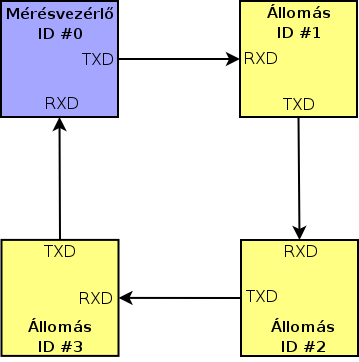
\includegraphics[width=60mm]{TokenRing.png}\end{center}
}

%%%%%%%%%%%%%%%%%%%%%%%%%%%%%%%%%%%%%%%%%%%%%%%%%%%%%%%%%%%%%%%%%%%%%%%%%%%%%%%%%%%%%%%%%%%%%%%%%%%%%%%%%%%%%%%%%%%%

\frame[label=exampleframe]{
    \frametitle{A mérőhálózat és a berendezések főbb összetevői}

    \begin{itemize}
        \item Mérésvezérlő: személyi számítógép Linux-szal és a megfelelő működtető szoftverrel
        \pause
        \item Műszerek felépítése:
        \pause
        \begin{itemize}
            \item Processzor modul (mikrovezérlő és kisegítő áramkörei), ez tartja a kapcsolatot a mérésvezérlővel
            \pause
            \item Végrehajtó, beavatkozó és érzékelő szerveket tartalmazó modul
        \end{itemize}
    \end{itemize}
}

%%%%%%%%%%%%%%%%%%%%%%%%%%%%%%%%%%%%%%%%%%%%%%%%%%%%%%%%%%%%%%%%%%%%%%%%%%%%%%%%%%%%%%%%%%%%%%%%%%%%%%%%%%%%%%%%%%%%

%\frame[label=exampleframe]{
%    \frametitle{Az irányítástechnika területei}

%    \begin{itemize}
%        \item Vezérlés
%        \pause
%        \item Mérésadatgyűjtés
%        \pause
        %\item Transzfer karakterisztika felvétele
        %\pause
%        \item Szabályozás $\rightarrow$ kapcsoló üzemű tápegység
        %\pause
        %\item Tranziens állapotbeli vizsgálat
        %\pause
        %\item $\dots$
%    \end{itemize}
%}

%%%%%%%%%%%%%%%%%%%%%%%%%%%%%%%%%%%%%%%%%%%%%%%%%%%%%%%%%%%%%%%%%%%%%%%%%%%%%%%%%%%%%%%%%%%%%%%%%%%%%%%%%%%%%%%%%%%%

\frame[label=exampleframe]{
    \frametitle{A mérőberendezés blokkvázlata}
    \begin{center}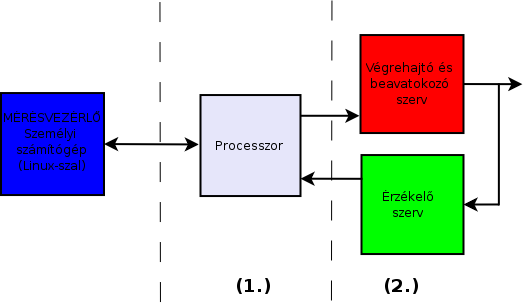
\includegraphics[width=100mm]{Blokk1.png}\end{center}
}

%%%%%%%%%%%%%%%%%%%%%%%%%%%%%%%%%%%%%%%%%%%%%%%%%%%%%%%%%%%%%%%%%%%%%%%%%%%%%%%%%%%%%%%%%%%%%%%%%%%%%%%%%%%%%%%%%%%%

\section{Hardver}

\frame[label=exampleframe]{
    \frametitle{Elvárások a mérésvezérlővel szemben}

    \begin{itemize}
        \item Operációs rendszer (Linux) és működtető (felhasználói) szoftver
        \pause
        \item Párhuzamos (nyomtató) vagy USB csatlakozó a JTAG-hez
        \pause
        \item Soros port vagy USB $\rightarrow$ soros port átalakító
    \end{itemize}

    \hspace{10mm}

    \pause
    A működtető szoftverről még a ,,Fejlesztői környezet'' részben lesz szó.
}

%%%%%%%%%%%%%%%%%%%%%%%%%%%%%%%%%%%%%%%%%%%%%%%%%%%%%%%%%%%%%%%%%%%%%%%%%%%%%%%%%%%%%%%%%%%%%%%%%%%%%%%%%%%%%%%%%%%%

\frame[label=exampleframe]{
    \frametitle{Az ARM alapú mikrovezérlők}

    \begin{itemize}
        \item Eredetileg az ARM magot processzorok számára fejlesztették ki (Acorn PC-k, Apple iPod, Intel PDA-k)
        \pause
        \item Mára a mikrovezérlő-gyártók kedvelt processzora lett
        \pause
            \begin{itemize}
                \item 32 bites aritmetikai egységgel rendelkezik
                \pause
                \item 4 GBájt lineáris címtartomány
                \pause
                \item Kis fogyasztás (29,4~mA áramfelvétel 50~MHz-es órajelfrekvencián)
                \pause
                \item A gyártók nagyszámú külső eszközzel egészítették ki, így alakult ki a mikrovezérlő, az \textbf{egy lapkán felépített számítógép}
            \end{itemize}
    \end{itemize}
}

%%%%%%%%%%%%%%%%%%%%%%%%%%%%%%%%%%%%%%%%%%%%%%%%%%%%%%%%%%%%%%%%%%%%%%%%%%%%%%%%%%%%%%%%%%%%%%%%%%%%%%%%%%%%%%%%%%%%

\frame[label=exampleframe]{
    \frametitle{Az ARM alapú mikrovezérlők kiegészítő elemei}

    \begin{itemize}
        \item FLASH és RAM memória (8-512 kbájt)
        \pause
        \item Analóg--digitális és digitális--analóg átalakító (10~bites)
        \pause
        \item 16 és 32 bites számlálók (események számlálására, időzítésre, PWM-re)
        \pause
        \item SPI: Serial Peripheral Interface, MMC és SD kártyák programozására
        \pause
        \item Megszakításvezérlő
        \pause
        \item Órajel-generátor
        \pause
        \item GPIO: általános célú (digitális) adatbemenetek és kimenetek
        \pause
        \item RTC: valós idejű óra
        \pause
        \item WDT: watchdog timer
    \end{itemize}
}

%%%%%%%%%%%%%%%%%%%%%%%%%%%%%%%%%%%%%%%%%%%%%%%%%%%%%%%%%%%%%%%%%%%%%%%%%%%%%%%%%%%%%%%%%%%%%%%%%%%%%%%%%%%%%%%%%%%%

\frame[label=exampleframe]{
    \frametitle{Az ARM alapú mikrovezérlők kiegészítő elemei (folytatás)}

    \begin{itemize}
        \item U(S)ART: univerzális aszinkron (soros) adó-vevő; ezt fogjuk a számítógéppel való kommunikációhoz használni
        \pause
        \item USB: univerzális soros busz
        \pause
        \item Ethernet
        \pause
        \item CAN és LIN busz: mikrovezérlők helyi hálózatba kötésére
    \end{itemize}
}

%%%%%%%%%%%%%%%%%%%%%%%%%%%%%%%%%%%%%%%%%%%%%%%%%%%%%%%%%%%%%%%%%%%%%%%%%%%%%%%%%%%%%%%%%%%%%%%%%%%%%%%%%%%%%%%%%%%%

\frame[label=exampleframe]{
    \frametitle{A választás}

    A tápegység megépítéséhez az ATMEL cég AT91SAM7S64 típusú mikrovezérlőjét használtam.
}

%%%%%%%%%%%%%%%%%%%%%%%%%%%%%%%%%%%%%%%%%%%%%%%%%%%%%%%%%%%%%%%%%%%%%%%%%%%%%%%%%%%%%%%%%%%%%%%%%%%%%%%%%%%%%%%%%%%%

\frame[label=exampleframe]{
    \frametitle{A processzor modul}

    A processzor modul tartalmaz
    \pause
    \begin{itemize}
                \item stabilizált, túlfeszültség ellen védett tápegységet, max. 15~V bemenő feszültségig
                \pause
                \item nagypontosságú órajelforrást a pontos időzítésekhez, aszinkron soros átvitelhez
                \pause
                \item a JTAG kivezetéseket, 10 pólusú szalagkábel csatlakozón keresztül
                \pause
                \item a megfelelő üzemmódba lépést beállító kapocspárt (nyomkövetés vagy normál üzem)
                \pause
                \item hardver RESET kivezetést a mikrovezérlő esetleges kézi újraindításához
                \pause
                \item LED-eket a hibás és megfelelő állapotok jerlzésére
    \end{itemize}
}

%%%%%%%%%%%%%%%%%%%%%%%%%%%%%%%%%%%%%%%%%%%%%%%%%%%%%%%%%%%%%%%%%%%%%%%%%%%%%%%%%%%%%%%%%%%%%%%%%%%%%%%%%%%%%%%%%%%%

\frame[label=exampleframe]{
    \frametitle{A processzor modul}

    A processzor modull tartalmaz (folytatás)
    \pause
    \begin{itemize}
                \item (Token~Ring--)RS-232 kommunikációt lehetővé tevő kivezetéseket és illesztő áramköröket
                \pause
                \item 4 pólusú szalagkábel csatlakozóra kivezetett ki- és bemeneteket:
                \pause
                    \begin{itemize}
                        \item 3 db PWM kimenet
                        \pause
                        \item 2 $\times$ 3 db analóg bemenet
                        \pause
                        \item 3 $\times$ 2 db LED kimenet (előlapra kivezetve)
                    \end{itemize}
    \end{itemize}
}

%%%%%%%%%%%%%%%%%%%%%%%%%%%%%%%%%%%%%%%%%%%%%%%%%%%%%%%%%%%%%%%%%%%%%%%%%%%%%%%%%%%%%%%%%%%%%%%%%%%%%%%%%%%%%%%%%%%%

\frame[label=exampleframe]{
    \frametitle{A processzor modul kapcsolási rajza}
    \begin{center}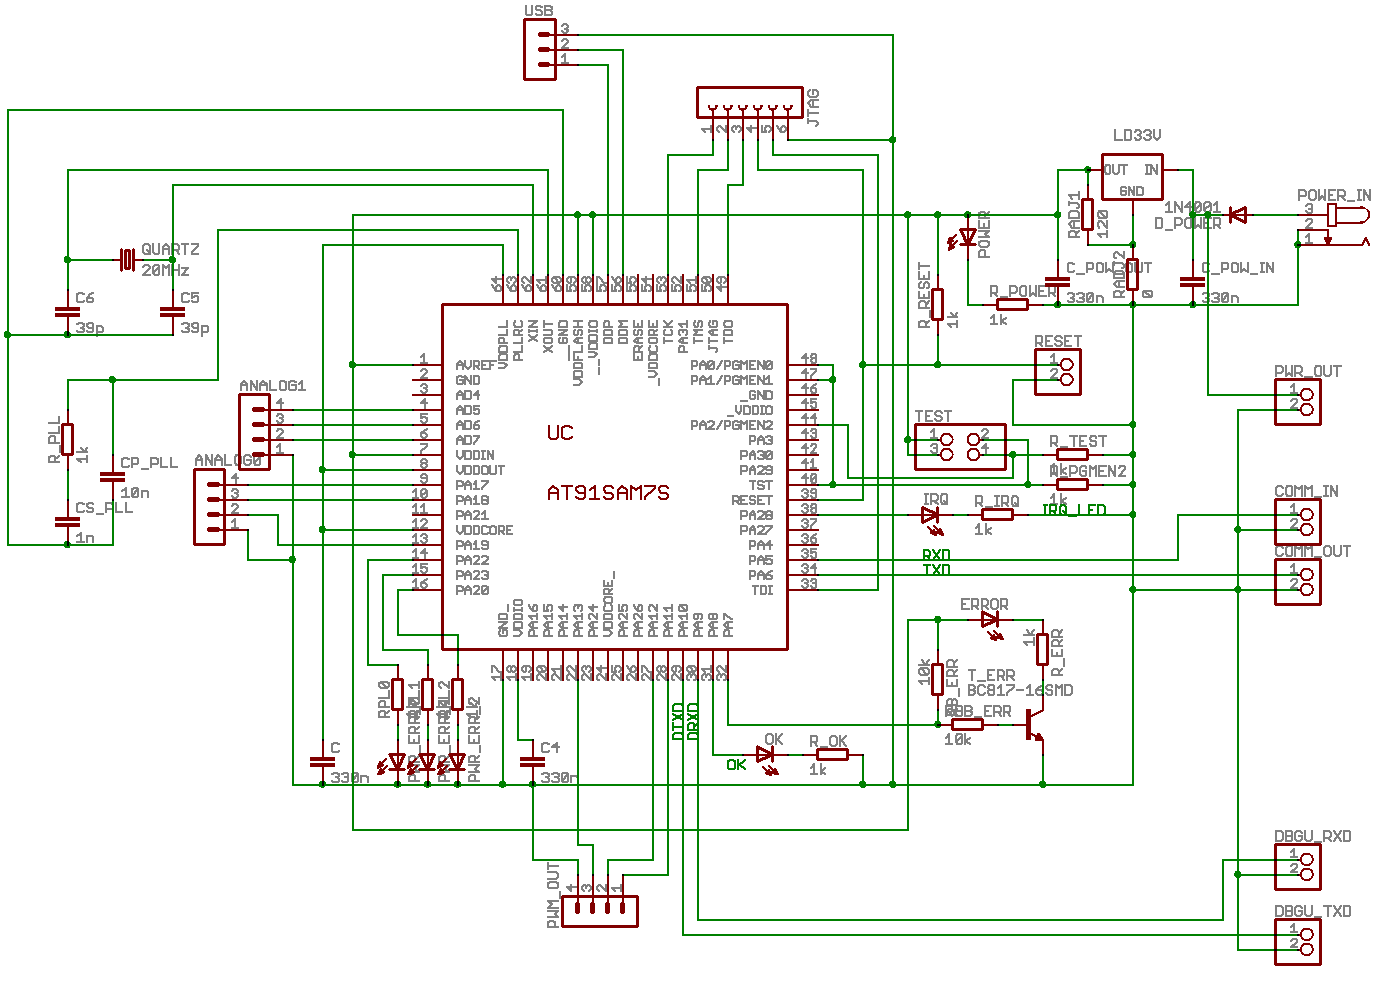
\includegraphics[width=90mm]{Proc_sch.png}\end{center}
}

%%%%%%%%%%%%%%%%%%%%%%%%%%%%%%%%%%%%%%%%%%%%%%%%%%%%%%%%%%%%%%%%%%%%%%%%%%%%%%%%%%%%%%%%%%%%%%%%%%%%%%%%%%%%%%%%%%%%
\frame[label=exampleframe]{
    \frametitle{A processzor modul NYÁK-rajza}
    \begin{center}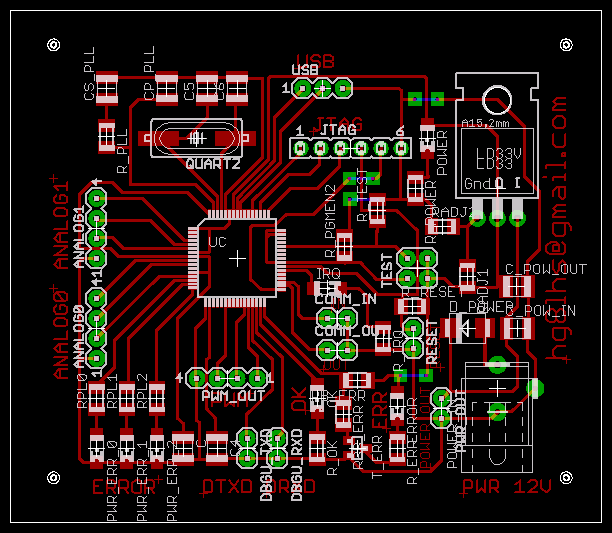
\includegraphics[width=70mm]{Proc_pcb.png}\end{center}
}

%%%%%%%%%%%%%%%%%%%%%%%%%%%%%%%%%%%%%%%%%%%%%%%%%%%%%%%%%%%%%%%%%%%%%%%%%%%%%%%%%%%%%%%%%%%%%%%%%%%%%%%%%%%%%%%%%%%%

\frame[label=exampleframe]{
    \frametitle{Érzékelő, végrehajtó és beavatkozó szervek}

    A modulon kaptak helyet
    \pause
    \begin{itemize}
        \item A kapcsolóeszközök (PWM jellel vezérelve)
        \pause
        \item Kimenő jelek mérésére szolgáló elemek (A/D átalakító segítségével, túlfeszültség-védetten)
    \end{itemize}
}

%%%%%%%%%%%%%%%%%%%%%%%%%%%%%%%%%%%%%%%%%%%%%%%%%%%%%%%%%%%%%%%%%%%%%%%%%%%%%%%%%%%%%%%%%%%%%%%%%%%%%%%%%%%%%%%%%%%%

\frame[label=exampleframe]{
    \frametitle{A végrehajtó-érzékelő modul kapcsolási rajza}
    \begin{center}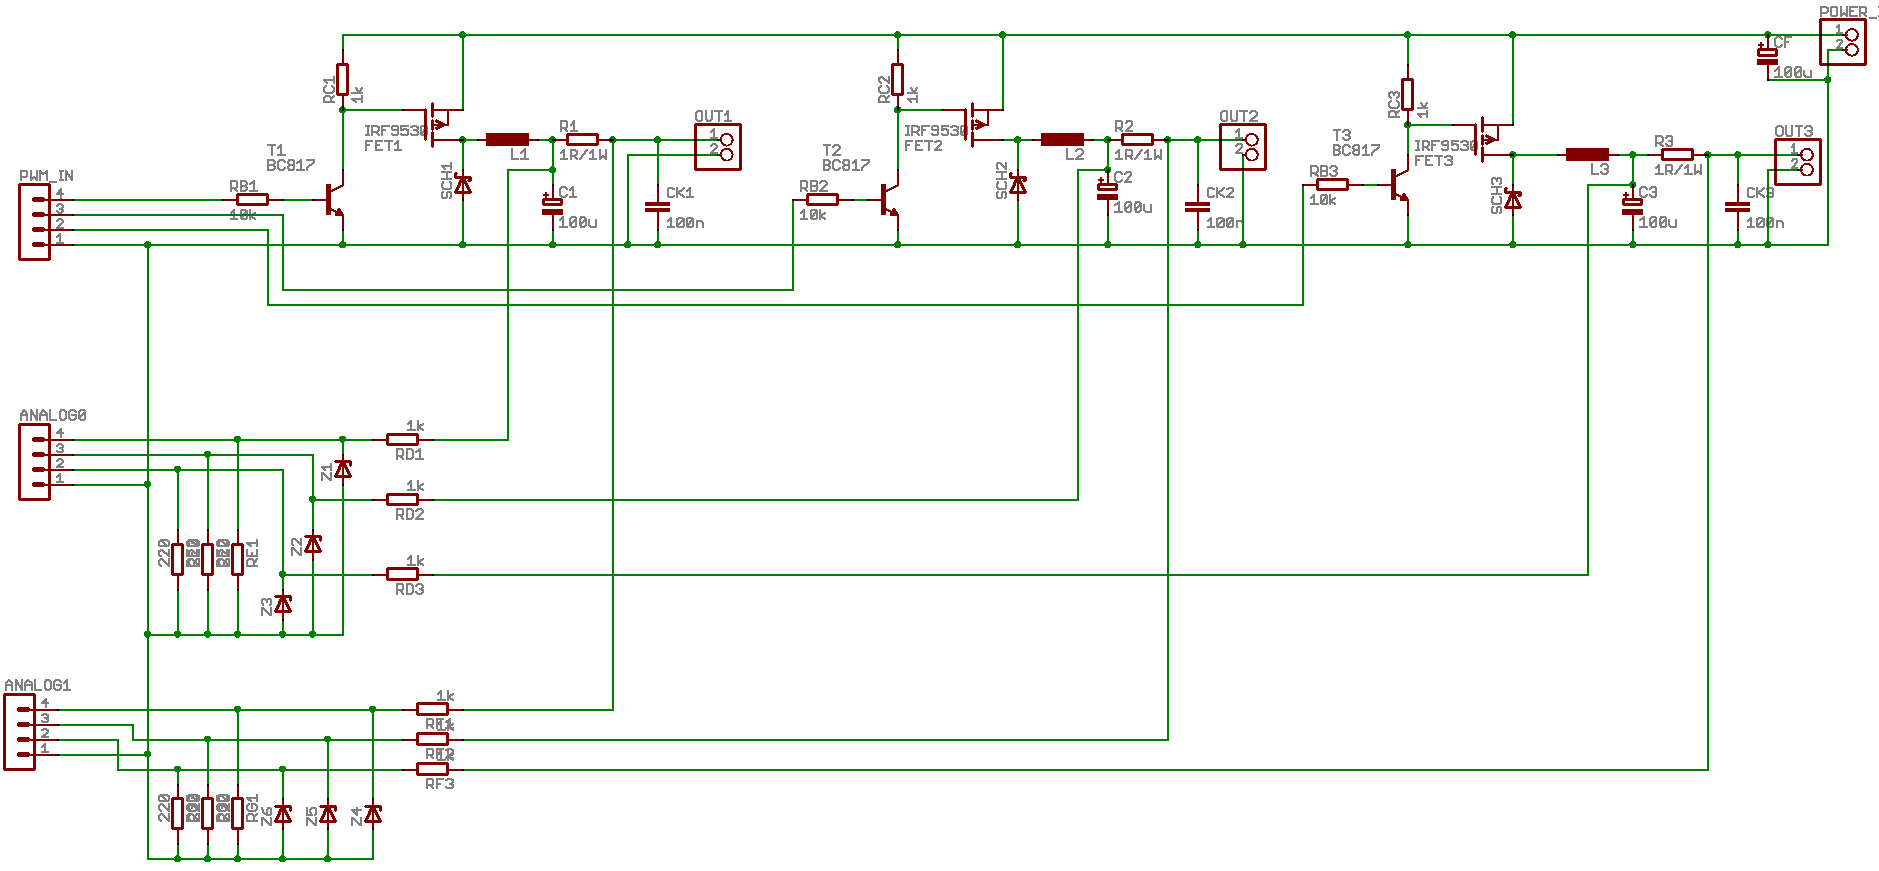
\includegraphics[width=110mm]{Power_sch.png}\end{center}
}

%%%%%%%%%%%%%%%%%%%%%%%%%%%%%%%%%%%%%%%%%%%%%%%%%%%%%%%%%%%%%%%%%%%%%%%%%%%%%%%%%%%%%%%%%%%%%%%%%%%%%%%%%%%%%%%%%%%%

\frame[label=exampleframe]{
    \frametitle{A végrehajtó-érzékelő modul NYÁK-rajza}
    \begin{center}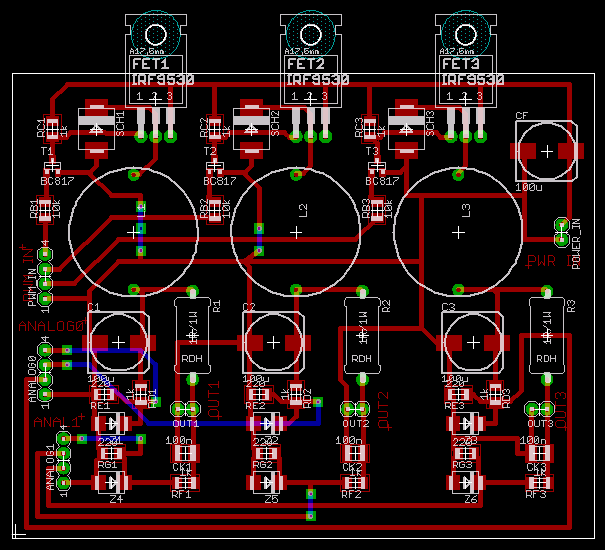
\includegraphics[width=70mm]{Power_pcb.png}\end{center}
}

%%%%%%%%%%%%%%%%%%%%%%%%%%%%%%%%%%%%%%%%%%%%%%%%%%%%%%%%%%%%%%%%%%%%%%%%%%%%%%%%%%%%%%%%%%%%%%%%%%%%%%%%%%%%%%%%%%%%

\section{Fejlesztői környezet}

\frame[label=exampleframe]{
    \frametitle{A fejlesztői környezet}

    A számítógép működtető szoftverének, és a mikrovezérlő programjának elkészítéséhez szükségesek a következő komponensek:\footnote{Erről részletesen a dolgozatban olvashatunk}
    \pause
    \begin{itemize}
        \item \texttt{binutils}, \texttt{gcc} és \texttt{gdb}: a számítógép számára fordítanak, ezekkel készül a mérésvezérlő szoftvere
        \pause
        \item \texttt{binutils}, \texttt{gcc} és \texttt{gdb}: ARM architektúrára fordítanak; segítségükkel állítjuk elő a mikrovezérlő programját (firmware)
        \pause
        \item \texttt{OpenOCD}: a számítógépen fut, feltöltő és nyomkövető program
    \end{itemize}
}

%%%%%%%%%%%%%%%%%%%%%%%%%%%%%%%%%%%%%%%%%%%%%%%%%%%%%%%%%%%%%%%%%%%%%%%%%%%%%%%%%%%%%%%%%%%%%%%%%%%%%%%%%%%%%%%%%%%%

\frame[label=exampleframe]{
    \frametitle{Adatátvitel soros porton keresztül}
    A számítógép és a mikrovezérlő között az átvitel bájtsoros és csomagorientált. Tulajdonságai:
    \pause
    \begin{itemize}
        \item Több eszköz (mérésvezérlő és mérőberendezések) kapcsolható rendszerbe
        \pause
        \item Fix csomagméret, előre definiált parancsok
        \pause
        \item Nincs szükség statikus eszközazonosítókra, ezeket a mérésvezérlő osztja ki
        \pause
        \item Hibavédelemmel ellátott a kommunikáció (8 bites ellenőrző összeg)
    \end{itemize}
}

%%%%%%%%%%%%%%%%%%%%%%%%%%%%%%%%%%%%%%%%%%%%%%%%%%%%%%%%%%%%%%%%%%%%%%%%%%%%%%%%%%%%%%%%%%%%%%%%%%%%%%%%%%%%%%%%%%%%

\frame[label=exampleframe]{
    \frametitle{Csomagformátum}
    \begin{itemize}
        \item (8~bit) Cél eszköz azonosítója (dinamikus)
        \item (8~bit) Parancs kódja 
        \item (8~bit) Adat, paraméter
        \item (8~bit) Ellenőrző összeg (nullázó bájt)
    \end{itemize}
}

%%%%%%%%%%%%%%%%%%%%%%%%%%%%%%%%%%%%%%%%%%%%%%%%%%%%%%%%%%%%%%%%%%%%%%%%%%%%%%%%%%%%%%%%%%%%%%%%%%%%%%%%%%%%%%%%%%%%

\frame[label=exampleframe]{
    \frametitle{A TokenRing--RS-232 hálózat felépítése}
    \begin{center}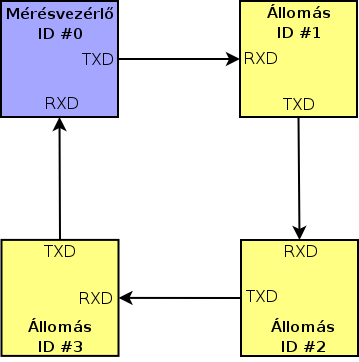
\includegraphics[width=60mm]{TokenRing.png}\end{center}
}

%%%%%%%%%%%%%%%%%%%%%%%%%%%%%%%%%%%%%%%%%%%%%%%%%%%%%%%%%%%%%%%%%%%%%%%%%%%%%%%%%%%%%%%%%%%%%%%%%%%%%%%%%%%%%%%%%%%%

\section{Felhasználói felületek}

\frame[label=exampleframe]{
    \frametitle{Vezérlő szoftver (felhasználói interfész)}
    \begin{center}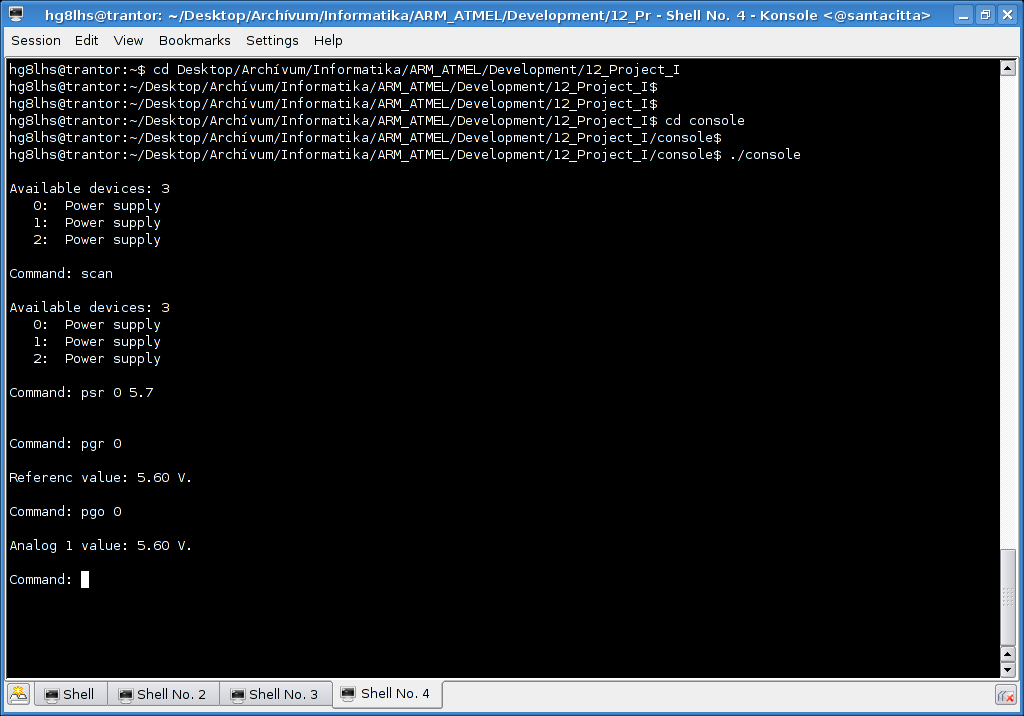
\includegraphics[width=100mm]{UI.png}\end{center}
}

%%%%%%%%%%%%%%%%%%%%%%%%%%%%%%%%%%%%%%%%%%%%%%%%%%%%%%%%%%%%%%%%%%%%%%%%%%%%%%%%%%%%%%%%%%%%%%%%%%%%%%%%%%%%%%%%%%%%

\frame[label=exampleframe]{
    \frametitle{Grafikus vezérlő szoftver}
    \begin{center}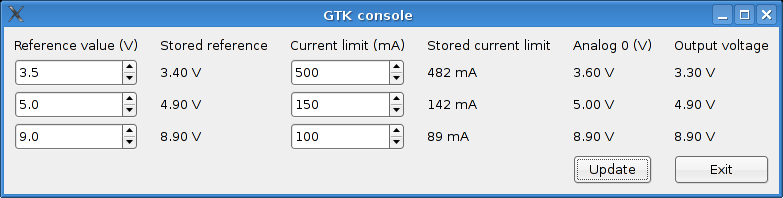
\includegraphics[width=110mm]{GUI.png}\end{center}
}

%%%%%%%%%%%%%%%%%%%%%%%%%%%%%%%%%%%%%%%%%%%%%%%%%%%%%%%%%%%%%%%%%%%%%%%%%%%%%%%%%%%%%%%%%%%%%%%%%%%%%%%%%%%%%%%%%%%%

\section{Utószó}

\frame[label=exampleframe]{
    \frametitle{Továbbfejlesztési lehetőségek}
    A dolgozatban megépített áramkör bővíthető, például
    \pause
    \begin{itemize}
        \item kifinomultabb szabályozással (PID kompenzált, véges beállású, stb.)
        \pause
        \item akkumulátor-töltő funkcióval
        \pause
        \item pontosabb kimenőáram-méréssel
        \pause
        \item további kommunikációs megoldásokkal (LIN, CAN, Ethernet, EtherCAT, GSM) $\dots$
    \end{itemize}
}

%%%%%%%%%%%%%%%%%%%%%%%%%%%%%%%%%%%%%%%%%%%%%%%%%%%%%%%%%%%%%%%%%%%%%%%%%%%%%%%%%%%%%%%%%%%%%%%%%%%%%%%%%%%%%%%%%%%%

\frame[label=exampleframe]{
    \frametitle{}
    \begin{center}
        \huge{\textbf{Kérdések?}}
    \end{center}
}

%%%%%%%%%%%%%%%%%%%%%%%%%%%%%%%%%%%%%%%%%%%%%%%%%%%%%%%%%%%%%%%%%%%%%%%%%%%%%%%%%%%%%%%%%%%%%%%%%%%%%%%%%%%%%%%%%%%%

\frame[label=exampleframe]{
    \frametitle{}
    \begin{center}
        \Huge{\textbf{Köszönöm a figyelmet!}}
    \end{center}
}

%%%%%%%%%%%%%%%%%%%%%%%%%%%%%%%%%%%%%%%%%%%%%%%%%%%%%%%%%%%%%%%%%%%%%%%%%%%%%%%%%%%%%%%%%%%%%%%%%%%%%%%%%%%%%%%%%%%%

\frame[label=exampleframe]{
    \frametitle{Felhasznált irodalom}
        \begin{itemize}
            \item \textit{ARM7TDMI~Technical~Reference~Manual~(Rev~3)}, ARM~Limited, 2001.
            \item \textit{AT91~ARM~Thumb-based~Microcontrollers}, ATMEL~Corporation, 2006.~november~22.
\end{itemize}
}

%%%%%%%%%%%%%%%%%%%%%%%%%%%%%%%%%%%%%%%%%%%%%%%%%%%%%%%%%%%%%%%%%%%%%%%%%%%%%%%%%%%%%%%%%%%%%%%%%%%%%%%%%%%%%%%%%%%%

\frame[label=exampleframe]{
    \frametitle{Felhasznált szoftverek}
        \begin{itemize}
            \item Ubuntu Linux 6.06 (Dapper Drake) [Linux kernel 2.6.15-27-k7]
            \item binutils 2.17 (using BFD version 2.17)
            \item gcc 4.0.3
            \item openocd -- Open On-Chip Debugger (2007-05-30 17:45 CEST)
            \item VIM --- VI IMproved version 6.4.6
            \item \LaTeX2$\varepsilon$ (pdfeTeX, Version 3.141592-1.21a-2.2)
            \item The GIMP 2.2.11
            \item aspell (International Ispell Version 3.1.20 (but really Aspell 0.60.4))
            \item Dia 0.94
            \item Eagle 4.16r2 for Linux, Light Edition
        \end{itemize}
}

%%%%%%%%%%%%%%%%%%%%%%%%%%%%%%%%%%%%%%%%%%%%%%%%%%%%%%%%%%%%%%%%%%%%%%%%%%%%%%%%%%%%%%%%%%%%%%%%%%%%%%%%%%%%%%%%%%%%

\end{document}
